%%
%% This is file `sample-sigconf.tex',
%% generated with the docstrip utility.
%%
%% The original source files were:
%%
%% samples.dtx  (with options: `all,proceedings,bibtex,sigconf')
%% 
%% IMPORTANT NOTICE:
%% 
%% For the copyright see the source file.
%% 
%% Any modified versions of this file must be renamed
%% with new filenames distinct from sample-sigconf.tex.
%% 
%% For distribution of the original source see the terms
%% for copying and modification in the file samples.dtx.
%% 
%% This generated file may be distributed as long as the
%% original source files, as listed above, are part of the
%% same distribution. (The sources need not necessarily be
%% in the same archive or directory.)
%%
%%
%% Commands for TeXCount
%TC:macro \cite [option:text,text]
%TC:macro \citep [option:text,text]
%TC:macro \citet [option:text,text]
%TC:envir table 0 1
%TC:envir table* 0 1
%TC:envir tabular [ignore] word
%TC:envir displaymath 0 word
%TC:envir math 0 word
%TC:envir comment 0 0
%%
%% The first command in your LaTeX source must be the \documentclass
%% command.
%%
%% For submission and review of your manuscript please change the
%% command to \documentclass[manuscript, screen, review]{acmart}.
%%
%% When submitting camera ready or to TAPS, please change the command
%% to \documentclass[sigconf]{acmart} or whichever template is required
%% for your publication.
%%
%%
\documentclass[sigconf]{acmart}
\usepackage[font=small,skip=0pt]{caption}
\usepackage{comment}
\usepackage{pgf}
%\usepackage{layouts}
\usepackage{booktabs}
\usepackage{soul}
\usepackage{booktabs}
\usepackage{footnote}
\usepackage{threeparttable}
\usepackage{multirow}
\usepackage{makecell}
\usepackage{color, colortbl}
\hyphenation{cost-ef-fi-cien-cy}

%%
%% \BibTeX command to typeset BibTeX logo in the docs
\AtBeginDocument{%
  \providecommand\BibTeX{{%
    Bib\TeX}}}

%% Rights management information.  This information is sent to you
%% when you complete the rights form.  These commands have SAMPLE
%% values in them; it is your responsibility as an author to replace
%% the commands and values with those provided to you when you
%% complete the rights form.

\copyrightyear{2026}
\acmYear{2026}
\setcopyright{cc}
\setcctype{by}
\acmConference[ACM Sustainability Week Companion '26]{ACM Sustainability Week 2026}{June 22--25, 2026}{Banff, AB, Canada}
\acmBooktitle{ACM Sustainability Week 2026 (ACM Sustainability Week Companion '26), June 22--25, 2026, Banff, AB, Canada}
\acmDOI{10.1145/3765611.3815015}
\acmISBN{979-8-4007-2199-1/2026/06}

%%
%% Submission ID.
%% Use this when submitting an article to a sponsored event. You'll
%% receive a unique submission ID from the organizers
%% of the event, and this ID should be used as the parameter to this command.
%%\acmSubmissionID{123-A56-BU3}

%%
%% For managing citations, it is recommended to use bibliography
%% files in BibTeX format.
%%
%% You can then either use BibTeX with the ACM-Reference-Format style,
%% or BibLaTeX with the acmnumeric or acmauthoryear sytles, that include
%% support for advanced citation of software artefact from the
%% biblatex-software package, also separately available on CTAN.
%%
%% Look at the sample-*-biblatex.tex files for templates showcasing
%% the biblatex styles.
%%

%%
%% The majority of ACM publications use numbered citations and
%% references.  The command \citestyle{authoryear} switches to the
%% "author year" style.
%%
%% If you are preparing content for an event
%% sponsored by ACM SIGGRAPH, you must use the "author year" style of
%% citations and references.
%% Uncommenting
%% the next command will enable that style.
%%\citestyle{acmauthoryear}


%%
%% end of the preamble, start of the body of the document source.
\begin{document}

%%
%% The "title" command has an optional parameter,
%% allowing the author to define a "short title" to be used in page headers.
\title[Towards Uncovering Indoor Satisfaction Profiles]{Towards Uncovering Indoor Satisfaction Profiles: LLM Capacity for Structured Extraction from Occupant Feedback}
% LLM-enhanced workplace occupant profile development from a large-scale survey databas

%%
%% The "author" command and its associated commands are used to define
%% the authors and their affiliations.
%% Of note is the shared affiliation of the first two authors, and the
%% "authornote" and "authornotemark" commands
%% used to denote shared contribution to the research.
\author{Thomas Parkinson}
\email{thomas.parkinson@sydney.edu.au}
\orcid{0000-0002-0088-8754}
\affiliation{%
  \institution{The University of Sydney}
  \city{Sydney}
  \country{Australia}
 }

\author{Stefano Schiavon}
\email{schiavon@berkeley.edu}
\orcid{0000-0003-1285-5682}
\affiliation{%
  \institution{University of California, Berkeley}
  \city{Berkeley}
  \country{USA}
 }

 \author{Wenhao Zhang}
\email{wenhao.zhang@u.nus.edu}
\orcid{0009-0007-0093-6916}
\affiliation{%
  \institution{National University of Singapore}
  \city{Singapore}
  \country{Singapore}
 }


\author{Clayton Miller}
\email{cmiller@smu.edu.sg}
\orcid{0000-0002-1186-4299}
\affiliation{%
  \institution{Singapore Management University}
  \city{Singapore}
  \country{Singapore}
}

%%
%% By default, the full list of authors will be used in the page
%% headers. Often, this list is too long, and will overlap
%% other information printed in the page headers. This command allows
%% the author to define a more concise list
%% of authors' names for this purpose.
\renewcommand{\shortauthors}{Parkinson, et al.}

%%
%% The abstract is a short summary of the work to be presented in the
%% article.
\begin{abstract} % 150-250 words 
\hspace{\parindent} 
Local large language models (LLM) offer a scalable, privacy-preserving approach to extracting structured attributes from free text from built environment occupant surveys, but there is little guidance on what model capacity is needed for reliable extraction. We address this gap with a validation study comparing three locally deployed LLM models (3B, 8B, 27B parameters) on structured complaint-style extraction from 6,283 post-occupancy evaluation survey narratives focused on categories of indoor environmental quality. The 3B model produces near-random classifications ($\kappa$ < 0.15), the 8B model achieves only slight to fair agreement ($\kappa$ = 0.05--0.33), and the 27B model reaches moderate agreement with human coding ($\kappa$ = 0.44--0.58). We contextualise this finding within a reproducible pipeline that integrates latent profile analysis of 16 indoor environmental satisfaction items (n = 39,149), identifying eight occupant profiles, with LLM-based extraction of complaint tone, severity, attribution, and work impact. A classification benchmark shows that neither text content nor LLM-extracted features predict profile membership beyond chance, establishing that satisfaction profiles and complaint text capture independent constructs. This work prototypes a framework for the forensic characterization of the diversity of personal subjective experience in indoor built environments.
\end{abstract}

%%
%% The code below is generated by the tool at http://dl.acm.org/ccs.cfm.
%% Please copy and paste the code instead of the example below.
\begin{CCSXML}
<ccs2012>
   <concept>
       <concept_id>10010147.10010178.10010179</concept_id>
       <concept_desc>Computing methodologies~Natural language processing</concept_desc>
       <concept_significance>500</concept_significance>
       </concept>
   <concept>
       <concept_id>10003120.10003121.10011748</concept_id>
       <concept_desc>Human-centered computing~Empirical studies in HCI</concept_desc>
       <concept_significance>300</concept_significance>
       </concept>
   <concept>
       <concept_id>10002951.10003227.10003351.10003444</concept_id>
       <concept_desc>Information systems~Clustering</concept_desc>
       <concept_significance>300</concept_significance>
       </concept>
 </ccs2012>
\end{CCSXML}

\ccsdesc[500]{Computing methodologies~Natural language processing}
\ccsdesc[300]{Human-centered computing~Empirical studies in HCI}
\ccsdesc[300]{Information systems~Clustering}

%%
%% Keywords. The author(s) should pick words that accurately describe
%% the work being presented. Separate the keywords with commas.
\keywords{large language models, structured text extraction, model validation, post-occupancy evaluation, occupant satisfaction}
%%
%\received{24 April 2026}
%\received[revised]{09 October 2025}
%\received[accepted]{09 October 2025}
%% This command processes the author and affiliation and title
%% information and builds the first part of the formatted document.
\maketitle

%%%%%%%%%%%%%%%%%%%%%%%%%%%%%%%%%%%%%%%%%%%%%%%%%%%%%%%%%%%%%%%%%%%%%%%%%%%%%%%%
\section{Introduction}
\label{sec:intro}

Research in indoor environmental quality in the built environment traditionally focuses on discovering \emph{generally} what creates comfort and productivity for building occupants. However, emerging evidence from the subfields of thermal, aural, and visual comfort indicates that building occupants exhibit significant personal differences in how they perceive indoor environments \cite{Kim2018-tu,Quintana2023-ik}. These studies have made progress towards this characterization but suffer from relatively small sample sizes, frequently fewer than 100 people. 

Post-occupancy evaluation (POE) surveys have been around for decades and typically provide large cross-sectional datasets, albeit with no longitudinal breadth and a rigid structure \cite{graham2021}. These surveys typically collect two data streams: structured satisfaction ratings across environmental domains and optional free-text responses where occupants share their subjective experience (usually complaints) in a specific environment in their own words. The quantitative data are well-studied, but the qualitative data remain under-exploited \cite{graham2021}. Manual thematic analysis does not scale to the tens of thousands of responses in large POE databases, and automated approaches have been limited to topic modeling or keyword extraction \cite{Moezzi01042011}, which struggle with the short, domain-specific text characteristic of occupant feedback.

Recent advances in locally deployable large language models (LLMs) offer a scalable approach to extract structured attributes from unstructured text \cite{hayes2025, player2025}, yet there is little empirical guidance on what model capacity is needed for reliable extraction in this domain. The domain classification of occupant complaints (e.g., acoustic vs. thermal) is based on content keywords \cite{sadick2025}. Extracting pragmatic attributes such as tone or severity requires inference about communicative intent, which is a harder task that may require greater model capacity. Meanwhile, person-centered methods such as latent profile analysis (LPA) can identify subgroups of occupants with different satisfaction patterns \cite{spurk2020}. To our knowledge, the integration of LPA with LLM-based text analysis of occupant feedback has not yet been explored in built-environment research. Combining LPA with LLM-based text analysis could reveal whether satisfaction subgroups differ in how they communicate dissatisfaction, but only if the text extraction is reliable.

We address these gaps with a reproducible pipeline implemented in R using the \texttt{targets} workflow manager. Our contributions are: (1) a validation study comparing three locally deployed models of increasing capacity (3B, 8B, and 27B parameters) against human coding, providing practical guidance on minimum model capacity for structured extraction; (2) a classification benchmark testing whether text features (content-based or LLM-extracted) can predict satisfaction profile membership; and (3) an eight-profile LPA solution characterizing distinct occupant satisfaction signatures, which serves as the downstream context for the text analysis. All analysis code and the extraction pipeline are available for replication.

% \subsection{}
% \hspace{\parindent} 

%%%%%%%%%%%%%%%%%%%%%%%%%%%%%%%%%%%%%%%%%%%%%%%%%%%%%%%%%%%%%%%%%%%%%%%%%%%%%%%%
\section{Methods}
\subsection{Data}
We used the University of California, Berkeley's Center for the Built Environment (CBE) Occupant Survey database \cite{graham2021}, filtering to US office buildings. The database contains satisfaction ratings on 7-point scales across indoor environmental and workspace domains, workspace configuration indicators, and optional free-text responses across nine question types (layout, acoustics, thermal comfort, lighting, air quality, cleanliness, furnishings, cleaning services, and general building comments).

For LPA, we selected 16 indoor environmental satisfaction items spanning space, visual privacy, ease of interaction, furniture comfort, furniture adjustability, temperature, air quality, light amount, visual comfort, noise level, sound privacy, cleanliness, cleaning service, maintenance, building overall, and workspace overall. From 56,197 respondents, listwise deletion of incomplete satisfaction data yielded 39,149 complete cases (30.3\% excluded). For text analysis, the corpus comprised over 41,000 responses; we processed a stratified sample of up to 100 responses per profile per question type (N = 6,283) to ensure representation across all profiles and complaint domains. The analysis workflow is summarised in Figure \ref{fig:workflow}.

\begin{figure*}[!htb]
\begin{center}
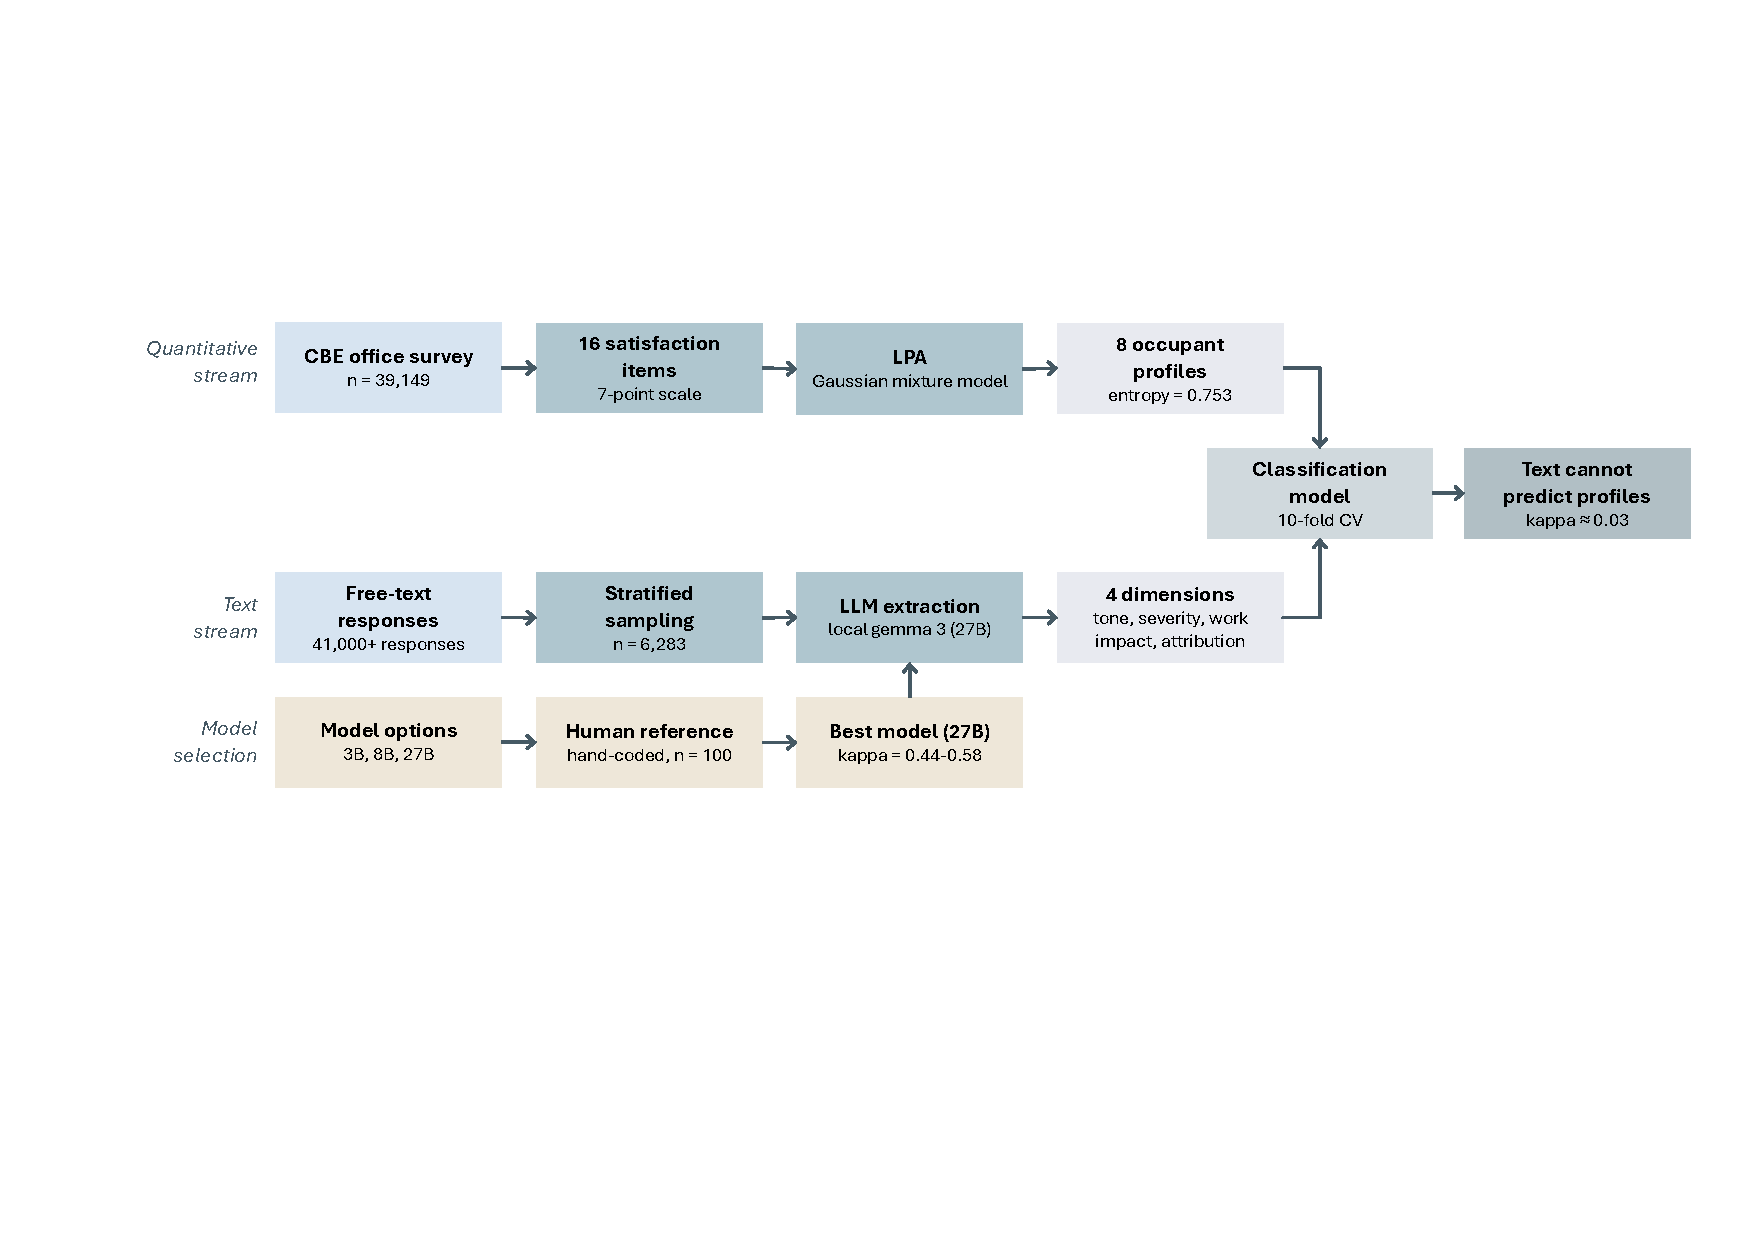
\includegraphics[width=0.9\textwidth, trim= 0cm 0cm 0cm 0cm,clip]{img/pipeline_architecture.pdf}
\Description{Analysis pipeline diagram with two parallel streams. The quantitative stream derives eight occupant profiles from latent profile analysis of 16 satisfaction items (n = 39,149). The text stream applies stratified sampling and LLM extraction to yield four complaint-style dimensions from 6,283 free-text responses. A validation branch compares three local models (3B, 8B, 27B parameters) against human coding; a classification benchmark tests whether text features predict profiles.}
\caption{Analysis pipeline. The quantitative stream derives eight occupant profiles from LPA of 16 satisfaction items (n = 39,149). The text stream applies stratified sampling and LLM extraction to yield four complaint-style dimensions from 6,283 free-text responses. A validation branch compares three local models (3B, 8B, 27B) against human coding; a classification benchmark tests whether text features predict profiles.}
\label{fig:workflow}
\end{center}
\end{figure*}

\subsection{Latent Profile Analysis}
We estimated latent solutions with 1 to 10 profiles using Gaussian mixture modelling in R (\texttt{mclust}). For each solution, \texttt{mclust} compared a range of covariance structures and selected the best-fitting one based on the Bayesian information criterion (BIC) \cite{spurk2020}. From the 2-profile solution onward, the preferred structure was EEV, indicating ellipsoidal profiles with equal volume and shape. We recorded the Bayesian information criterion, integrated completed likelihood (ICL), entropy, and average posterior probability for each solution. We then assessed the robustness of these solutions using split-half cross-validation, repeating the procedure 20 times for each number of profiles and comparing the resulting classifications with the adjusted Rand index. Bootstrap likelihood ratio tests (BLRTs) were run with 100 bootstrap samples on a stratified subsample (n = 5,001) rather than the full dataset, because full-sample BLRTs were computationally impractical at this scale. In addition, in very large samples BLRTs often continue to favor models with one additional profile. Consistent with this, in our case, the BLRT supported the solution with one additional profile at every comparison tested (all $p < .01$). To assess the external validity of the profiles, we used multinomial logistic regression, with the largest profile treated as the reference group, to examine whether profile membership was associated with workspace type and person-level variables (hours worked per week and tenure).

\subsection{LLM-Enhanced Text Analysis}
We extracted four complaint-style dimensions from each response using constrained LLM prompts via the `mall` R package interfacing with Ollama:
\begin{itemize}
    \item Tone: negative (frustrated, resigned, urgent) vs. non-negative (neutral, constructive)
    \item Severity: significant (moderate, severe) vs. minor
    \item Attribution: building, HVAC, colleagues, management, equipment, layout, other
    \item  Work impact: concentration, communication, productivity, health, comfort, none
\end{itemize}

Prompts enforced single-token responses from predefined vocabularies to ensure parseable outputs. Five dimensions were initially extracted, but coping was excluded from analysis because the survey structure elicits complaints by design, producing insufficient variation for discrimination. Tone and severity were collapsed to binary categories after validation indicated finer-grained distinctions were unreliable. All primary extraction used temperature 0.0; sensitivity checks at temperatures 0.0, 0.1, and 0.5 showed minimal change in aggregate distributions.

\subsection{Validation}
We evaluated three locally deployed open-source models: llama3.2 (3B parameters), llama3.1 (8B parameters), and gemma3 (27B parameters), all served via Ollama. A stratified random sample of 100 responses was independently coded by a single human annotator using the same taxonomy. For each model and extraction dimension, agreement between the model output and the human annotations was quantified using Cohen’s kappa, with 95\% confidence intervals estimated from 2,000 bootstrap replicates. To aid interpretation, we described kappa values using the conventional Landis and Koch benchmarks: slight (0.00--0.20), fair (0.21--0.40), moderate (0.41--0.60), substantial (0.61--0.80), and almost perfect (0.81--1.00) agreement. Values near zero were interpreted as indicating chance-level agreement. We acknowledge that a single coder cannot separate LLM error from human subjectivity; the kappa values reported thus reflect agreement with one human interpretation rather than reliability against a consensus standard.

To test whether text-derived features could predict profile membership, we compared four feature sets using regularised multinomial logistic regression with the \texttt{glmnet} package in R under 10-fold stratified cross-validation: (A) TF-IDF document-term vectors (top 500 terms), (B) LDA topic proportions (gamma), (C) text embeddings (768-dimensional ``nomic-embed-text'' vectors reduced to 46 principal components retaining 80\% of variance), and (D) LLM-extracted complaint-style dimensions (dummy-coded). We report accuracy, macro-averaged F1, and Cohen's $\kappa$; chance accuracy for eight classes is 12.5\%.

\section{Results}

\subsection{Model Capacity Determines Extraction Quality}
The validation study revealed a clear relationship between model size and extraction quality (Table \ref{tab:agreement} \& Figure \ref{fig:validation}). The 3B-parameter model (llama3.2) produced classifications that were essentially random across all dimensions ($\kappa$ < 0.15). The 8B model (llama3.1) showed slight to fair agreement, with performance varying by dimension: tone classification remained near random ($\kappa$ = 0.05) while severity ($\kappa$ = 0.31), attribution ($\kappa$ = 0.27), and work impact ($\kappa$ = 0.33) reached fair agreement. The 27B model (gemma3) achieved moderate agreement with the human coder: $\kappa$ = 0.54 for tone, 0.44 for severity, 0.58 for attribution, and 0.52 for work impact. Among the three models tested, only the 27B model achieved agreement levels sufficient for population-level analysis, suggesting that model capacity is a binding constraint for structured extraction from short occupant text. Temperature sensitivity checks (temperatures 0.0, 0.1, 0.5) showed stable aggregate distributions, indicating that extraction was robust to sampling temperature within this range.

% Requires: \usepackage{booktabs}
\begin{table}[ht]
    \centering
    \footnotesize
    \caption{Inter-rater agreement (Cohen's $\kappa$) between LLM and human coding (n = 100) by model size. 95\% CIs for the 8B model ranged from [0.01, 0.11] (tone) to [0.15, 0.47] (severity).}
    \label{tab:agreement}

    \newcolumntype{L}[1]{>{\raggedright\arraybackslash}m{#1}}
    \newcolumntype{C}[1]{>{\centering\arraybackslash}m{#1}}

    \begin{tabular}{L{1.0cm} C{1.0cm} C{1.1cm} C{1.1cm} C{1.2cm} C{1.0cm}}
        \toprule
        \multirow{2}{*}{\raisebox{-1.5ex}{\makecell[l]{Model}}} &
        \multirow{2}{*}{\raisebox{-1.5ex}{\makecell[c]{Params}}} &
        \multicolumn{4}{c}{Cohen's $\kappa$} \\
        \cmidrule(lr){3-6}
        & & Tone & Severity & Attribution & Impact \\
        \midrule
        llama3.2 & 3B  & $<$0.15 & $<$0.15 & $<$0.15 & $<$0.15 \\
        llama3.1 & 8B  & 0.05    & 0.31    & 0.27    & 0.33    \\
        gemma3   & 27B & 0.54    & 0.44    & 0.58    & 0.52    \\
        \bottomrule
    \end{tabular}
\end{table}
% %%%%%%%%%%%%%%%%%%%%%%%%%%%%%%%%%%%%%%%%%%%%%%%%%%%%%%%%%%%%%%%%%%%%%%%%%%%%%%%%
\begin{figure}[ht]
    \centering
    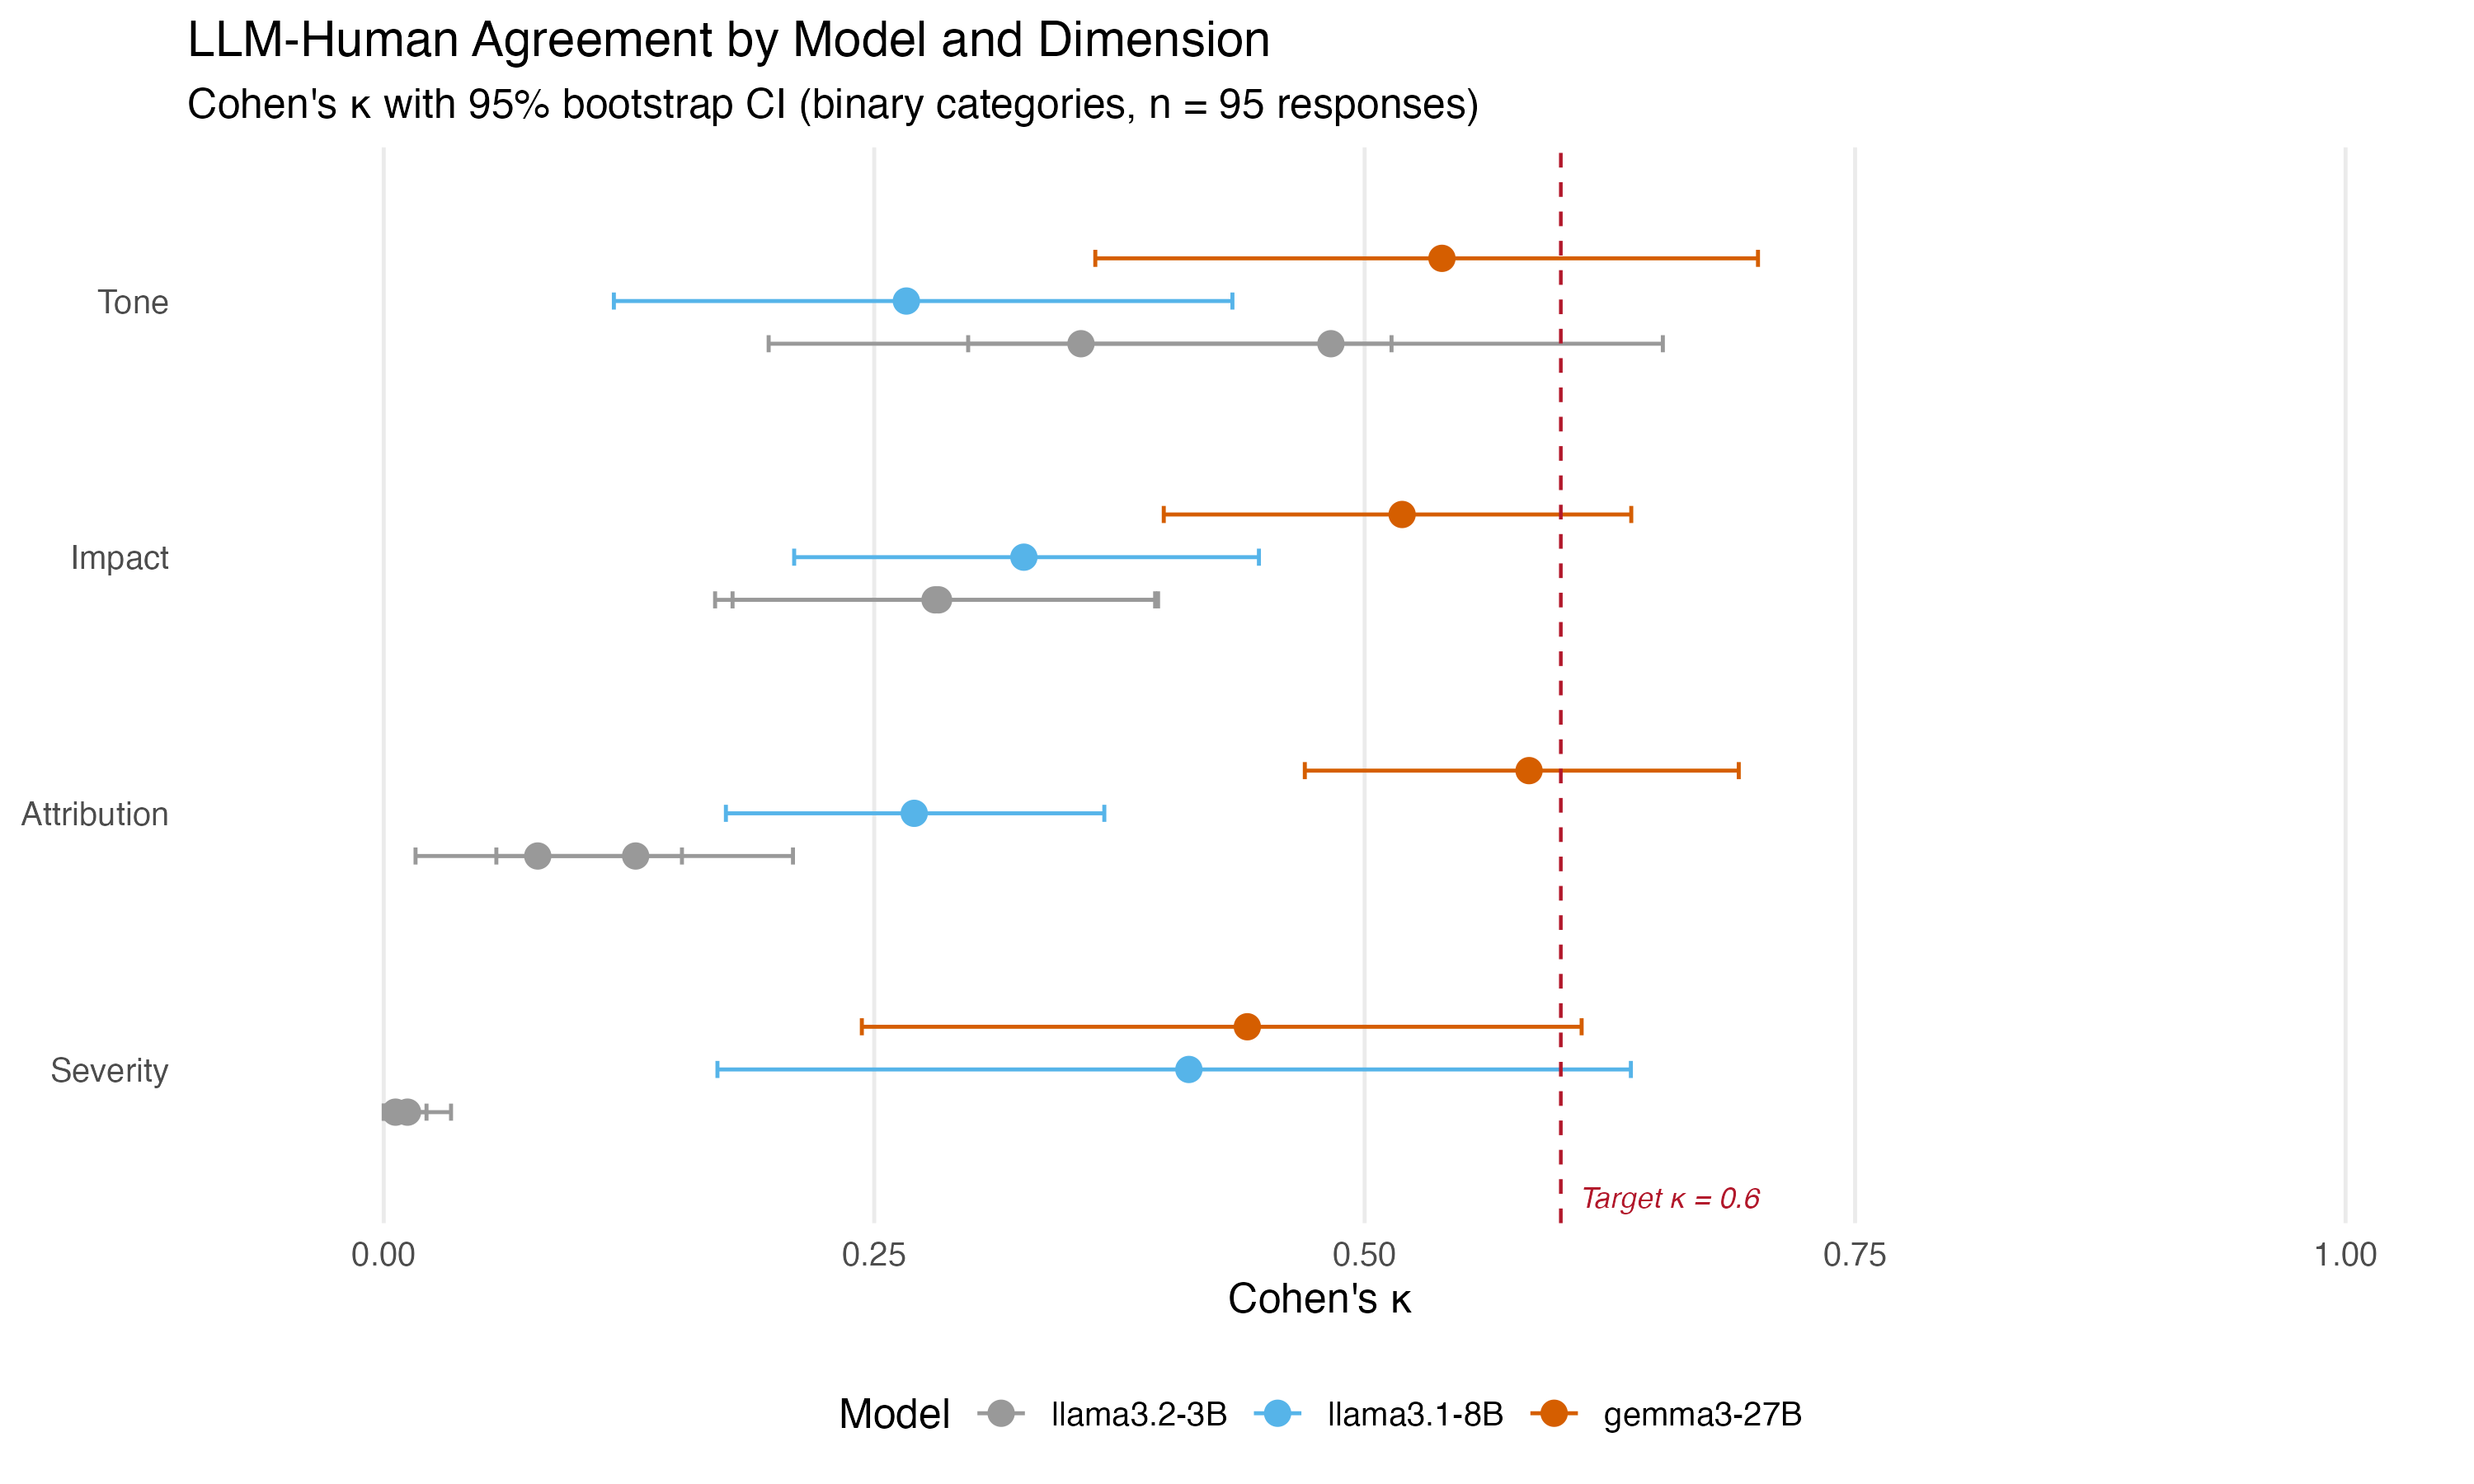
\includegraphics[width=\linewidth]{img/6_validation_kappa.png}
    \Description{Bar chart of Cohen's kappa by model size (3B, 8B, 27B parameters) and extraction dimension (tone, severity, attribution, work impact). The 27B model achieves the highest kappa values across dimensions. Error bars show 95\% bootstrap confidence intervals.}
    \caption{Cohen's kappa by model size and extraction dimension. Error bars show 95\% bootstrap confidence intervals.}
    \label{fig:validation}
\end{figure}

\subsection{Eight Latent Satisfaction Profiles}
LPA identified an eight-profile EEV solution (entropy = 0.753, average posterior probability = 0.793). We note that entropy falls below the 0.80 benchmark sometimes recommended for LPA \cite{spurk2020}, indicating moderate classification uncertainty for some individuals. We observed that BIC improved monotonically as the number of profiles increased, whereas improvements in ICL became smaller beyond the six-profile solution. The selected solution balanced classification quality, interpretability, and split-half stability (adjusted Rand index 0.21--0.30 for six to ten profiles). Table \ref{tab:lpa} summarizes the profiles.

\begin{table}[ht]
    \centering
    \footnotesize
    \setlength{\tabcolsep}{3pt}
    \renewcommand{\arraystretch}{1.10}
    \caption{Latent satisfaction profiles (n = 39,149). Satisfaction items were rated from 1 (very dissatisfied) to 7 (very satisfied). The Open Plan Acoustic Crisis profile scored at the scale minimum (1.0) for sound privacy. Selected items are shown; full profile means are provided in the supplementary materials.}
    \label{tab:lpa}

    \newcolumntype{L}[1]{>{\raggedright\arraybackslash}m{#1}}
    \newcolumntype{C}[1]{>{\centering\arraybackslash}m{#1}}

    \newcommand{\RowStrut}{\rule{0pt}{2.8ex}}

    \begin{tabular}{L{1.7cm} C{0.7cm} C{0.6cm} C{0.9cm} C{0.6cm} C{1.2cm} C{1.3cm}}
        \toprule
        Profile &
        N &
        \% &
        \raisebox{0.0ex}{\shortstack[c]{Sound\\privacy}} &
        Noise &
        \raisebox{0.0ex}{\shortstack[c]{Workspace\\overall}} &
        Maintenance \\
        \midrule
        \RowStrut Generally Satisfied & 11{,}418 & 29.2 & 4.2 & 5.1 & 5.9 & 6.0 \\
        \RowStrut Moderate Satisfaction & 11{,}171 & 28.5 & 3.3 & 4.3 & 4.8 & 5.3 \\
        \RowStrut Private Office Satisfied & 5{,}604 & 14.3 & 4.2 & 4.9 & 5.7 & 4.8 \\
        \RowStrut Open Plan Acoustic Crisis & 5{,}219 & 13.3 & 1.0 & 1.6 & 2.9 & 4.2 \\
        \RowStrut Building Systems Dissatisfied & 2{,}153 & 5.5 & 3.2 & 4.1 & 4.2 & 2.5 \\
        \RowStrut Clean but Uncomfortable & 1{,}704 & 4.4 & 3.2 & 4.3 & 4.6 & 4.5 \\
        \RowStrut Well-Maintained Moderate & 1{,}593 & 4.1 & 3.2 & 4.3 & 4.7 & 5.4 \\
        \RowStrut Maintenance Crisis & 287 & 0.7 & 3.7 & 4.3 & 4.8 & 2.8 \\
        \bottomrule
    \end{tabular}
\end{table}

Acoustics and privacy were the primary differentiators. The \textit{Open Plan Acoustic Crisis} profile was dominated by open-plan workstations (75\% open-plan), and multinomial regression confirmed that open-plan configurations increased odds of membership by 5--6 times relative to enclosed private offices. Hours worked per week remained significant after controlling for workspace type (OR = 1.33 per standard deviation), indicating that exposure duration contributes beyond physical configuration.

\subsection{Text and Ratings Capture Orthogonal Constructs}
All feature sets performed near chance level for predicting profile membership from complaint text (Table \ref{tab:membership} \& Figure \ref{fig:classification}), establishing that satisfaction profiles and complaint text capture different information about occupant experience.

% Requires: \usepackage{booktabs}
\begin{table}[ht]
    \centering
    \footnotesize
    \caption{Classification of profile membership from text features. 10-fold
    stratified cross-validation with regularized multinomial logistic regression.
    Chance accuracy = 12.5\%}
    \label{tab:membership}
    \begin{tabular}{p{2.0cm} p{1.7cm} p{1.7cm} p{1.7cm}}
        \toprule
        Feature set & Accuracy & Macro F1 & Cohen's $\kappa$ \\
        \midrule
        A: TF-IDF         & $0.160 \pm 0.004$ & $0.132 \pm 0.004$ & $0.026 \pm 0.005$ \\
        B: LDA gamma      & $0.159 \pm 0.004$ & $0.139 \pm 0.006$ & $0.023 \pm 0.005$ \\
        C: Embeddings     & $0.162 \pm 0.004$ & $0.147 \pm 0.006$ & $0.027 \pm 0.005$ \\
        D: LLM dimensions & $0.162 \pm 0.004$ & $0.152 \pm 0.011$ & $0.025 \pm 0.004$ \\
        E: Combined       & $0.166 \pm 0.004$ & $0.126 \pm 0.004$ & $0.032 \pm 0.005$ \\
        \bottomrule
    \end{tabular}
\end{table}

\begin{figure}[ht]
    \centering
    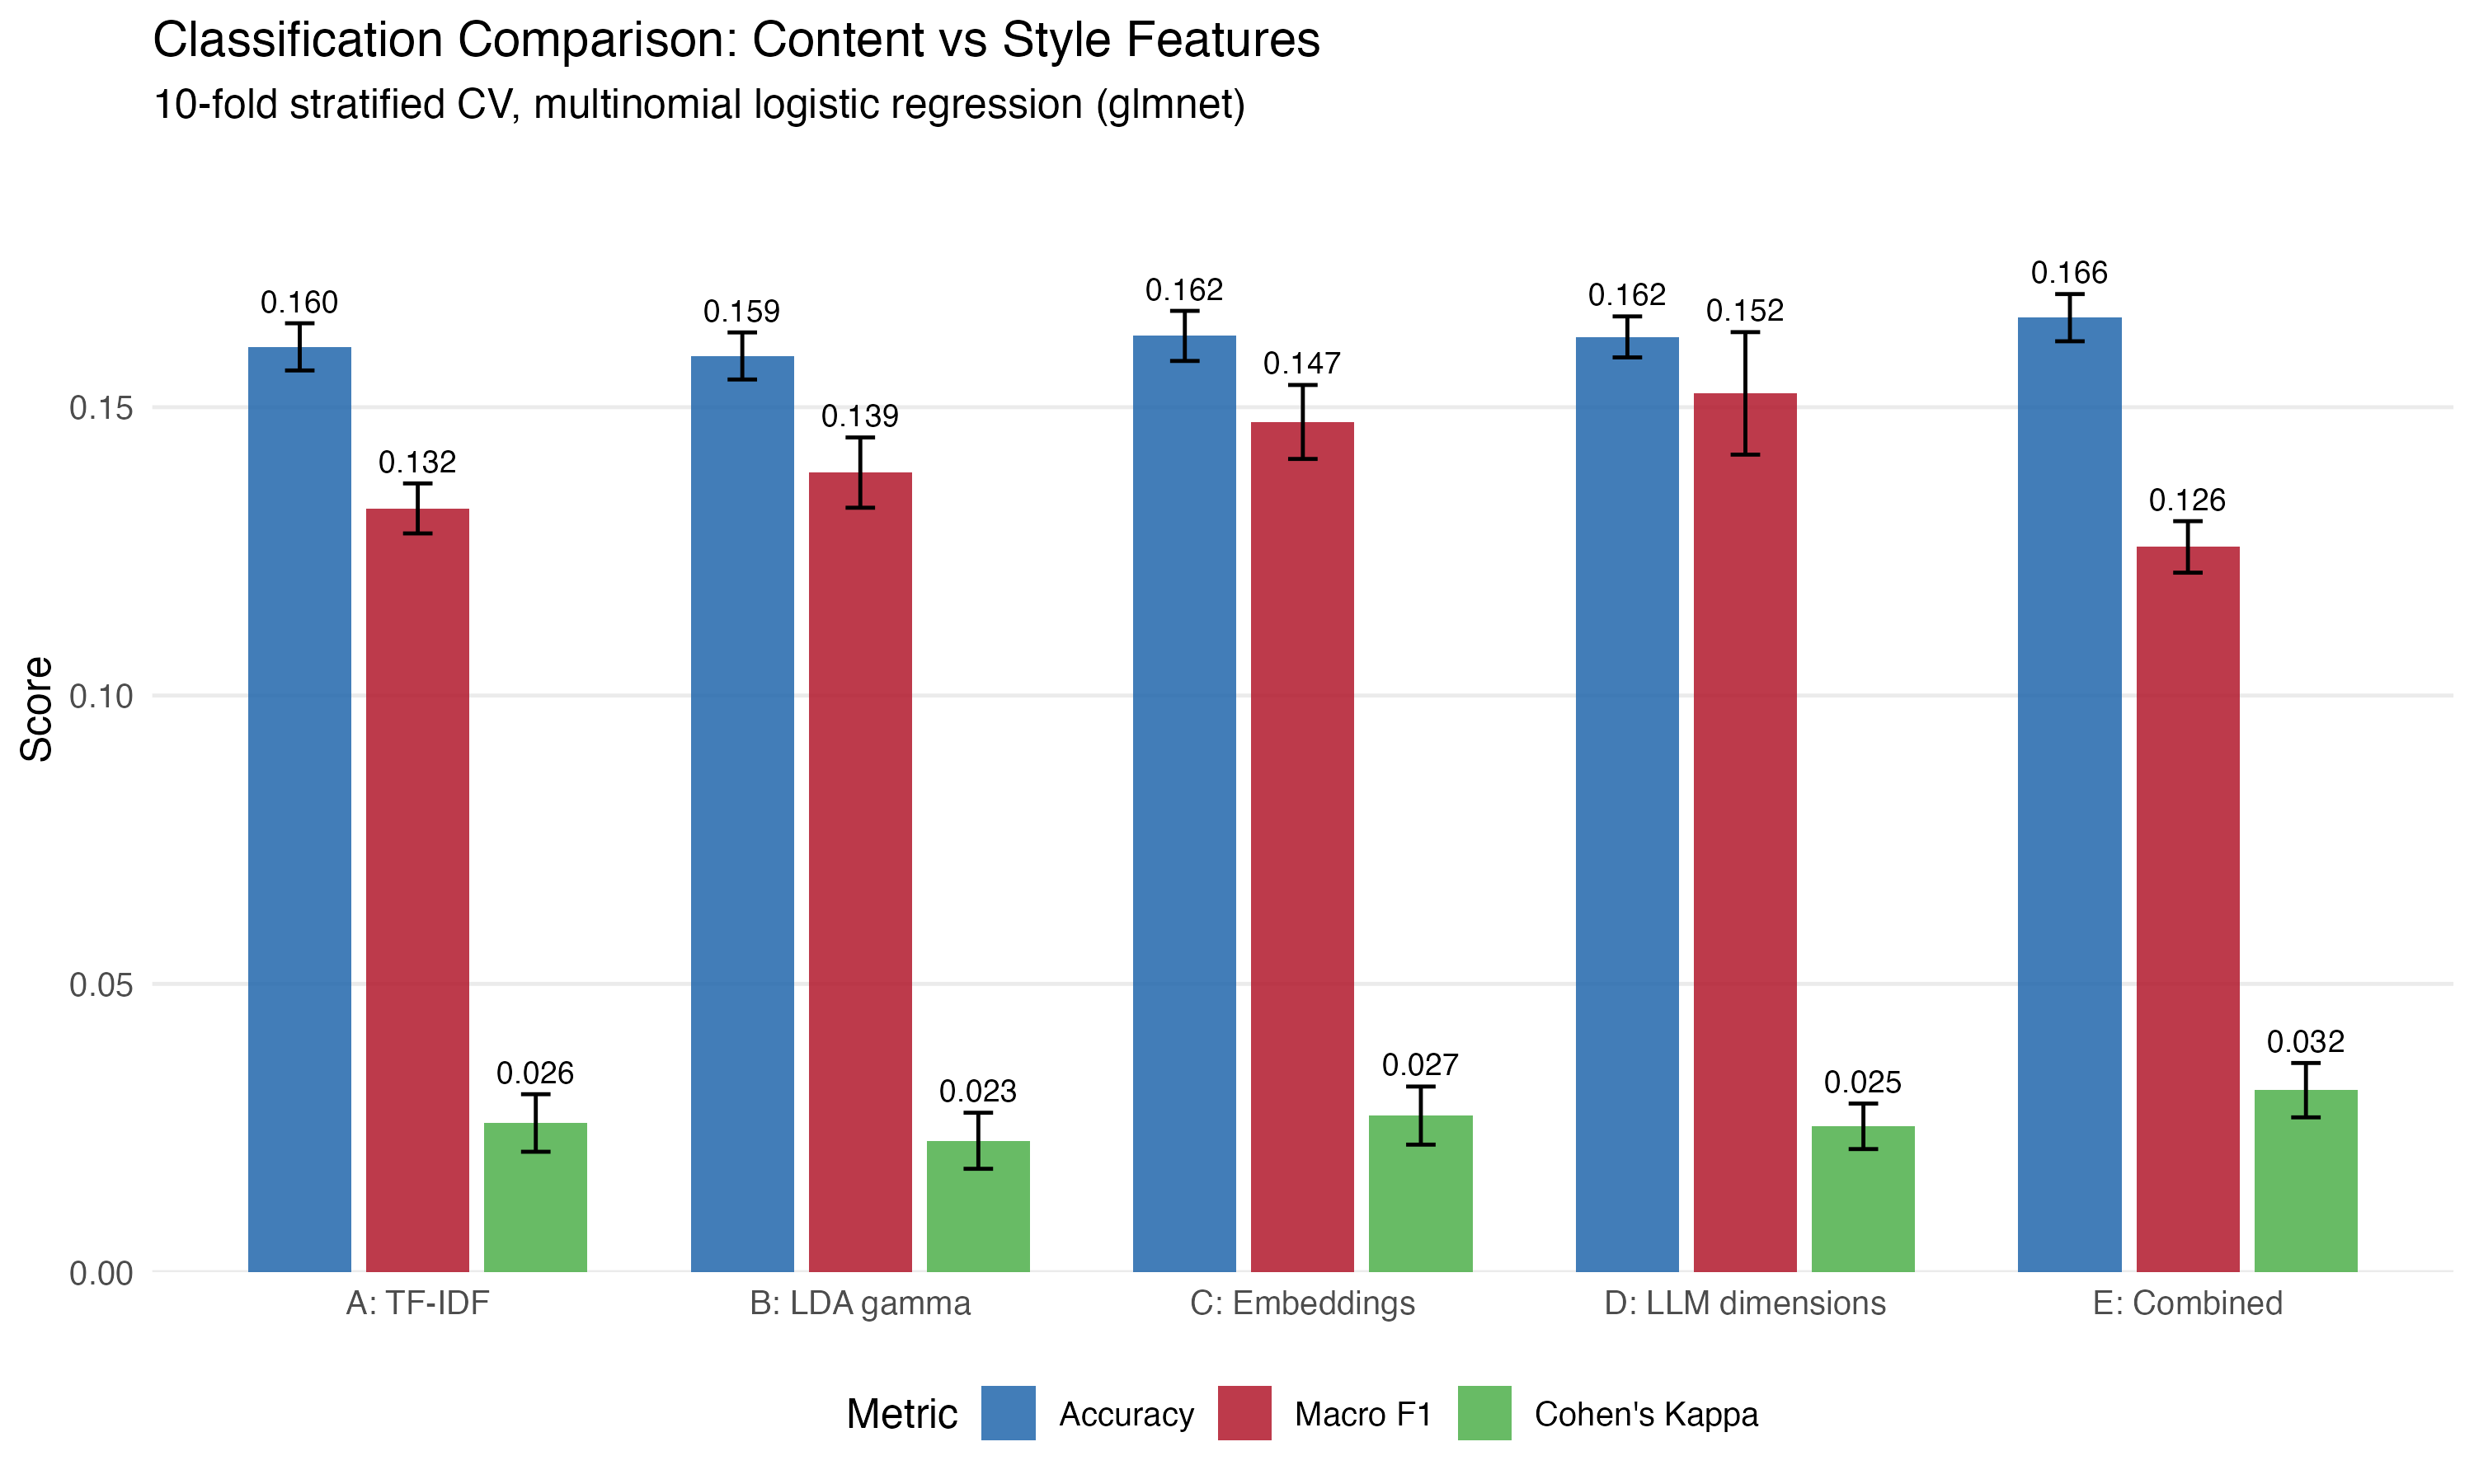
\includegraphics[width=\linewidth]{img/8_classification_comparison.png}
    \Description{Bar chart comparing classification performance across five feature representations: bag-of-words (TF-IDF), topic proportions (LDA), dense embeddings, and structured LLM extractions. Accuracy, macro F1, and Cohen's kappa all cluster near the 12.5\% chance baseline, indicating near-zero predictive value across all representations.}
    \caption{Classification performance by feature set (10-fold stratified CV). Accuracy, macro F1, and Cohen's $\kappa$ cluster near the 12.5\% chance baseline across all five representations. The visual uniformity rules out representation choice as an explanation for the null result.}
    \label{fig:classification}
\end{figure}

All models achieved $\kappa$ < 0.04, indicating near-zero predictive value. This consistency across four qualitatively different feature representations (bag-of-words (TF-IDF), topic proportions (LDA), dense embeddings, and structured LLM extractions) strengthens the conclusion that the signal is absent rather than missed by a particular representation. Satisfaction profiles are defined by rating patterns across 16 items, whereas complaint text appears to reflect a different aspect of occupant experience. Text-based methods should therefore not be expected to replace structured rating instruments for occupant segmentation.

\section{Discussion}

\subsection{Minimum model capacity for structured extraction}
The most actionable finding is the relationship between model capacity and extraction quality. Among the three models tested, the 3B model produced random outputs, the 8B model achieved only slight to fair agreement, and the 27B model reached moderate agreement ($\kappa$ = 0.44--0.58). We emphasize that three data points do not establish a general capacity threshold---a differently architected 8B model or a 14B model might perform differently. What our results do establish is that researchers deploying local LLMs for structured extraction from short, domain-specific text should not assume smaller models will suffice, and that empirical validation against human coding is essential regardless of model size. This aligns with broader evidence that structured extraction requiring pragmatic inference is harder than content-based topic classification \cite{sadick2025}.

\subsection{Text-rating orthogonality}
The classification null result is informative rather than negative. Near-chance performance across all feature representations establishes that satisfaction profiles and complaint narratives capture different aspects of occupant experience. Profiles are defined by patterns of satisfaction ratings across 16 environmental domains; complaint text conveys what bothers people and how they express it, but not their broader satisfaction pattern. This has implications for anyone attempting text-based occupant segmentation: complaint text alone is unlikely to recover the latent structure identified through rating instruments.

It also has practical implications for POE providers. Analysing satisfaction ratings alone may not provide a sufficiently actionable understanding of occupant experience, because the open-text comments capture concerns and expressions of dissatisfaction that are not reflected in the rating profiles. In practice, quantitative ratings and open-text feedback should therefore be analysed together. This finding may also have implications for building certification and evaluation frameworks that depend mainly on structured indicators, because narrative feedback may capture aspects of occupant experience that are not reflected in quantitative ratings alone.

\subsection{Towards characterizing individualized indoor satisfaction}
The technical ability for this approach to detect and segment clusters of perception of indoor environment have been explored and partially validated. This effort has produced promising evidence that this method could help better characterize what groups of perspectives building occupants fall into when experiencing indoor environments. Sources of text-based information from occupants can be found not only in POE surveys, but in web-based sources, social media, or reviews on website that rate the services that indoor environments might provide (i.e.: restaurants, retail, etc.). A significant limitation with the framework tested is in its inability to disentangle the impact of the unique perspective of the individual providing the information in the survey versus the conditions in the space itself. The CBE survey lacks a longitudinal or spatially diverse element where a participant is giving their perspective of a variety of spaces, which could facilitate this disentanglement.

\subsection{Limitations}
The moderate Cohen's $\kappa$ values (0.44--0.58) reflect the inherent difficulty of classifying subjective dimensions such as tone and severity from short text. This challenge is further compounded by the validation design: agreement was assessed against a single human coder, meaning that the reported $\kappa$ values conflate LLM error with individual human subjectivity. The validation sample (n = 100), while sufficient for estimating aggregate $\kappa$, also limits the assessment of per-category reliability, particularly for low-frequency categories. Future work should therefore incorporate multiple independent coders and larger validation samples to establish a more robust human-agreement baseline and assess category-level reliability. 

In addition, the LPA entropy (0.753) falls below the commonly recommended 0.80 threshold, indicating classification ambiguity that may propagate into subsequent analyses. Similarly, the classification benchmark relied on a single model (regularised logistic regression). Although more flexible nonlinear models could potentially capture additional signal, the consistently weak performance across diverse feature representations suggests that any such improvement would likely be limited. More broadly, the analysis is cross-sectional, and the CBE database may over-represent organisations that commission evaluations, which may limit the generalisability of the findings. 

\begin{sloppypar}
Finally, this study focuses on locally deployable open-source LLMs, selected to support reproducibility, cost efficiency, and privacy-preserving deployment in real-world building applications. As a result, we do not evaluate frontier proprietary models accessed through commercial APIs (e.g., OpenAI GPT-class models, Google Gemini Pro models, and Anthropic Claude Sonnet/Opus models), which may achieve stronger performance on nuanced text interpretation tasks. The reported results should therefore be interpreted as a conservative baseline under practical deployment constraints. Future work should systematically compare local and frontier models to better understand the performance–cost trade-offs.
\end{sloppypar}

\section{Conclusion and future work}
We present a reproducible R pipeline combining latent profile analysis with locally deployed LLM extraction for post-occupancy survey data. Our validation study provides practical guidance: among three models tested, only the 27B-parameter model achieved moderate agreement with human coding for structured extraction of complaint tone, severity, attribution, and work impact. Smaller models (3B, 8B) were inadequate for this task, and empirical validation against human coding is essential. The classification benchmark establishes that complaint text and satisfaction ratings capture orthogonal constructs, a finding with implications for text-based occupant segmentation. Future work should extend this initial validation by incorporating multi-annotator consensus labels, larger validation samples, and comparisons between locally deployed models and frontier proprietary models.

\section*{Reproducibility}
The full pipeline is implemented in R using \texttt{targets} for reproducibility and \texttt{mall} + Ollama for local, privacy-preserving LLM deployment. This work and its analysis can be reproduced using the data and code available in the GitHub repository\footnote{\url{https://github.com/IEQLab/office_profiler}}.

\begin{acks}
This research was partially supported by the Republic of Singapore’s National Research Foundation through the Campus for Research Excellence and Technological Enterprise (CREATE) program, and the industry consortium members of the Center for the Built Environment (CBE), University of California, Berkeley.
\end{acks}

%% The next two lines define the bibliography style to be used, and the bibliography file.
\bibliographystyle{ACM-Reference-Format}
\bibliography{references}

\end{document}